\documentclass{beamer}

\usepackage[italicdiff]{physics}
\usepackage{hyperref}
\usepackage{url}

\newcommand{\dbar}{d\hspace*{-0.08em}\bar{}\hspace*{0.1em}}
\renewcommand{\L}{\mathcal{L}}

\newenvironment{itemframe}[1]{\begin{frame}{#1}\begin{itemize}}   {\end{itemize}\end{frame}}

% Changes style of actual slides
\usetheme{Dresden}
% Changes color of slides
\usecolortheme{spruce}
% removes controls at bottom right side
\usenavigationsymbolstemplate{}

% for figures
\graphicspath{ {./figs/} }

\title{Functional Derivatives \& Lagrange Multipliers}
\author{Michael Cardiff}
\subtitle{PHYS 163a \ 09/20 Prep Work}

\begin{document}

\begin{frame}
  \titlepage
\end{frame}
\section{Functional Derivatives}
\begin{frame}{Functional Derivatives}
  We have met total derivatives, partial derivatives and more. Now what is this functional derivative?
  \begin{itemize}
  \item Works on functionals, which have functions as inputs, so they look like:
    \begin{align*}
      A[q]=\int_a^b f(r,q(r),\grad{q(r)})\dd{r}
    \end{align*}
  \item The functional derivative is a generalization of the Euler-Lagrange Equations:
    \begin{align*}
      \fdv{A}{q}=\pdv{f}{q}-\div{\pdv{f}{\grad{q}}}
    \end{align*}
  \end{itemize}
\end{frame}
\begin{frame}{Functional Derivatives}
  \begin{itemize}
  \item How do we find $\delta A$?
  \item Similar to the way we derive Euler-Lagrange Equations, only vary $q$:
    \begin{align*}
      \delta A&=\int_a^b\qty(\pdv{f}{q}\delta q(r)+\pdv{f}{\grad{q(r)}}
      \grad{\delta q(r)})\dd{r}\\
      &=\int_a^b\qty(\pdv{f}{q}\delta q(r)+\div{\pdv{f}{\grad{q(r)}}})
      \delta q(r)\dd{r}
    \end{align*}
  \item Therefore we can identify the parenthetical term as $\fdv{A}{q}$
  \end{itemize}
\end{frame}
\begin{frame}{Another Way}
  \begin{itemize}
  \item Define with an aribitrary function $\phi(x)$:
    \begin{align*}
      \int\fdv{F[\rho]}{\rho}(x)\phi(x)\dd{x}
    \end{align*}
  \item The derivative is then:
    \begin{align*}
      \int\fdv{F[\rho]}{\rho}(x)\phi(x)\dd{x}=\qty[\dv{\epsilon}
      F[\rho+\epsilon\phi]]_{\epsilon=0}
    \end{align*}
  \end{itemize}
\end{frame}
\begin{frame}{Why are they useful?}
  \begin{itemize}
  \item Probability theory makes use of functionals
  \item Functional derivative is how the functional changes with a certain change in the configuration, that is with a change in the input
  \item In order to get the least biased probability dostribution, we may need to minimize or maximize a functional
  \item This may require making use of the functional derivative.
  \end{itemize}
\end{frame}
\section{Lagrange Multipliers}
\begin{frame}{Lagrange Multipliers}
  \begin{itemize}
  \item Find extrema of a function $f(\vb{x})$ subject to constraints $g_i(\vb{x})=0$.
  \item Requirements of solution $\vb{x}_0$:
    \begin{itemize}
    \item Moving $\vb{x}$ in any direction increases $f(\vb{x})$ for minima and decreases $f(\vb{x})$ for maxima
    \item The constraints are obeyed: $g_i(\vb{x}_0)=0$ for all $i$
    \end{itemize}
  \item Go by example first to get intuition.
  \end{itemize}
\end{frame}
\begin{frame}{Lagrange Multiplier Example}
  \begin{columns}
    \begin{column}{0.5\textwidth}
      \begin{itemize}
      \item We want to find the maximum value of $f(x,y)=2x+y$ on the unit circle
      \item Identify function and constraints:
        \begin{gather*}
          f(x,y)=2x+y\\
          g(x,y)=x^2+y^2-1=0
        \end{gather*}
      \item Plot contours of $f(x,y)=k$ and $g(x,y)=0$
      \end{itemize}
    \end{column}
    \begin{column}{0.5\textwidth}
      \begin{figure}[H]
        \centering
        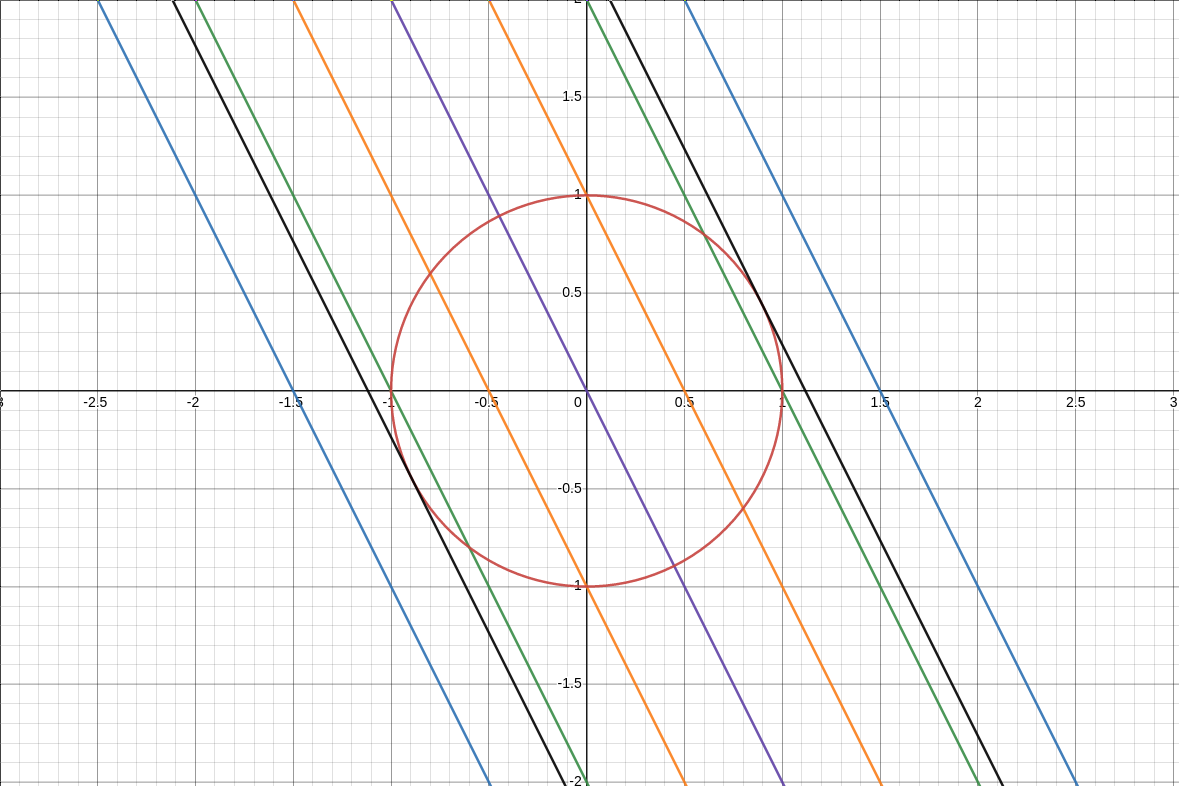
\includegraphics[width=5.0cm]{gradient1.png}
        \caption{Contours of $f$ and plot of $g(x,y)=0$}
      \end{figure}
    \end{column}
  \end{columns}
\end{frame}
\begin{frame}{Example Continued}
  \begin{itemize}
  \item Note increasing value of $k$ is moving the contour line to the right
  \item Notice the largest value of $k$ that still has a values on the red circle is the one that that is barely touches it without going over.
  \item In math talk, they are tangent. 
  \item Gradient can quantify this tangency.
  \end{itemize}
\end{frame}
\begin{frame}{Equations of Lagrange Multipliers}
  \begin{itemize}
  \item Gradients should be in the same direction at this point
  \item Not necessarily same rate, so introduce Lagrange multiplier $\lambda$, which quantifies this difference:
    \begin{align*}
      \grad{f(x,y)}=\lambda\grad{g(x,y)}
    \end{align*}
  \item This is only two equations, and now we have 3 unknowns
  \item The third equation will come from constraint!
    \begin{align*}
      g(x,y)=0
    \end{align*}
  \end{itemize}
\end{frame}
\section{Example}
\begin{frame}{Worked Out Example}
  \begin{itemize}
  \item Maximize $f(x,y)=2x+y$ on unit circle $x^2+y^2=1$
  \item Gradient of $f$ and $g$:
    \begin{gather*}
      \grad{f}=\ev{2,1}\\
      \lambda\grad{g}=\ev{2\lambda x,2\lambda y}
    \end{gather*}
  \item We can eliminate $x$ or $y$ using the constraint equation:
    \begin{align*}
      g(x,y)=0\implies x=\pm\sqrt{1-y^2}
    \end{align*}
  \item Then it is a simple system of equations:
    \begin{align*}
      \begin{cases}
        2=\pm2\lambda\sqrt{1-y^2}\\
        1=2\lambda y
      \end{cases}
    \end{align*}
  \end{itemize}
\end{frame}
\begin{frame}{Example Continued}
  \begin{itemize}
  \item The second equation yields:
    \begin{align*}
      \lambda=\frac1{2y}
    \end{align*}
  \item Subbing into the first:
    \begin{align*}
      2y=\pm\sqrt{1-y^2}
    \end{align*}
  \item Square both sides:
    \begin{align*}
      4y^2=1-y^2\implies \abs{y}=\frac1{\sqrt{5}}
    \end{align*}
  \item Using relationship between $x,y$:
    \begin{align*}
      x=\pm\sqrt{1-\qty(\frac1{\sqrt{5}})^2}=\pm\frac{2}{\sqrt{5}}
    \end{align*}
  \end{itemize}
\end{frame}
\begin{frame}{Answer?}
  \begin{itemize}
  \item Using some generality we got both the maxima and minima:
    \begin{align*}
      \ev{x,y}=\ev{\pm\frac2{\sqrt{5}},\pm\frac1{\sqrt{5}}}
    \end{align*}
  \item Giving a function value of $\pm\sqrt{5}$
  \end{itemize}
\end{frame}

\section{Takeaways}
\begin{frame}{Takeaways and Generalizations}
  \begin{itemize}
  \item A function is maximized with respect to another function when their gradients are in the same direction.
  \item Mathematically:
    \begin{align*}
      \grad{f}=\lambda\grad{g}
    \end{align*}
  \item This leads to $n$ equations where $f$ is a function of $n$ variables
  \item For each constraint you will get another $\lambda$, but the constraint equation provides an equation, giving a solveable system. 
  \end{itemize}
\end{frame}

\end{document}